% ============================================================================
%  Physical Review B -- version v3
%  Emergent altermagnetic correlations and d_xy pairing in the checkerboard
%  Hubbard model
%
%  Every number in this file traces to a file in the repository. Pointers are
%  given in comments beside each claim so the draft can be checked against data
%  rather than against memory. Items still needing input are marked TODO.
% ============================================================================
\documentclass[aps,prb,reprint,superscriptaddress,amsmath,amssymb,floatfix]{revtex4-2}

\usepackage{graphicx}
\usepackage{bm}

\renewcommand{\topfraction}{0.9}
\renewcommand{\bottomfraction}{0.8}
\renewcommand{\textfraction}{0.07}
\renewcommand{\floatpagefraction}{0.7}
\setcounter{topnumber}{3}
\setcounter{totalnumber}{4}

\begin{document}

\title{Emergent altermagnetic correlations in the checkerboard Hubbard model}

% TODO: author list and affiliations to be completed by the authors.
\author{[Author One]}
\affiliation{[Affiliation]}
\author{[Author Two]}
\affiliation{[Affiliation]}

\date{\today}

\begin{abstract}
We study magnetic correlations in the half-filled Hubbard model on the
checkerboard lattice by constrained-path quantum Monte Carlo. The hopping is
spin independent, so the momentum distributions of the two spin species coincide
at $U=0$ and any splitting must be generated by the interaction. The two
magnetic sublattices are exchanged by a fourfold rotation and by no translation,
which is the symmetry condition for a compensated spin splitting. We find such a
splitting above a finite interaction strength, with a momentum-space
polarization that is odd under $C_4$ and even under the diagonal mirror at all
126 interacting parameter sets studied, identifying the $d_{xy}$ channel. A
control at vanishing anisotropy, where the model reduces to the square lattice
and the splitting is forbidden, fixes the statistical floor of the estimator at
$6.3(2)\times10^{-4}$ per site, between 23 and 114 times below the measured
signal. Finite-size analysis on lattices from $8\times8$ to $16\times16$ sites
shows the equal-time structure factor falling as $1/N$ and the extrapolated
staggered moment dropping below the resolution of the calculation, so the
correlations remain short ranged on the lattices reached here.
\end{abstract}

\maketitle


% -------------------------------------------------------------------------
\section{Introduction}
% ---------------------------------------------------------------------------

Altermagnets combine a vanishing net moment with a spin-split band structure,
a combination long assumed to require either ferromagnetism or spin-orbit
coupling~\cite{Smejkal2022a,Smejkal2022b}. The splitting follows from the
crystal symmetry: the two opposite-spin sublattices are connected by a rotation
rather than by a translation or an inversion, so the spin degeneracy that a
conventional antiferromagnet enforces is absent.

Most microscopic models of this state build the splitting into the Hamiltonian,
usually through a spin-dependent hopping. The splitting is then present already
at zero interaction and the question of whether interactions alone can produce
it is left open. Two recent studies of the Lieb lattice state the gap directly,
noting that unbiased studies establishing an altermagnet as the ground state of
an interacting Hamiltonian are lacking~\cite{Kaushal2025,Duerrnagel2025}. Both
use methods with a controlled range of validity, unrestricted Hartree-Fock with
exact diagonalization on small clusters in the first case and a functional
renormalization group treatment of the weak-coupling limit in the second.

The checkerboard lattice offers a route to the same physics without putting it
in by hand. It is a square lattice with diagonal bonds on alternating
plaquettes, so the two sublattices are exchanged by a fourfold rotation about a
plaquette center but by no translation. The hopping is spin independent, and
the interaction is a uniform on-site Hubbard $U$. Any spin splitting therefore
appears only once magnetic correlations develop, which is the emergent route
rather than the built-in one.

We report constrained-path quantum Monte Carlo (CPQMC) calculations for this
model at half filling on lattices of $8\times8$ up to $16\times16$ sites. Three
results follow. The momentum-resolved spin polarization is nonzero above a
finite $U$ and has $d_{xy}$ symmetry at every interacting parameter set we
examined. A null calculation at vanishing anisotropy, where symmetry forbids the
signal, places the statistical floor two orders of magnitude below the measured
values. Finite-size analysis to $16\times16$ sites shows that the correlations
stay short ranged on the lattices reached, so we describe them as correlations
rather than as order.


% -------------------------------------------------------------------------
\section{Model and method}
% ---------------------------------------------------------------------------

We consider
\begin{equation}
H = \sum_{ij\sigma} t_{ij}\, c^{\dagger}_{i\sigma} c^{\phantom{\dagger}}_{j\sigma}
    + U \sum_i n_{i\uparrow} n_{i\downarrow},
\label{eq:H}
\end{equation}
with nearest-neighbor hopping $t_{ij} = t_0$ and diagonal hopping
$t_1 + t_2$ along $(1,1)$ and $t_1 - t_2$ along $(1,-1)$ on one sublattice, the
two exchanged on the other. Energies are in units of $|t_0|$, and we set
$t_0 = -1$ and $t_1 = 0.3$ throughout. The anisotropy is parametrized by
$\delta$ through $t_2 = -\delta$, so that $\delta = 0$ restores the plain square
lattice with uniform second-neighbor hopping and both sublattices become
equivalent. All calculations are at half filling.

The hopping in Eq.~(\ref{eq:H}) is spin independent by construction, so
$n_{\uparrow}(\bm{k}) = n_{\downarrow}(\bm{k})$ at $U = 0$ for every $\delta$.

We use CPQMC with a Trotter step $\Delta\tau = 0.01$, a projection length
$\beta = 32$, and $N_w = 1000$ walkers. The constrained-path approximation
introduces a bias controlled by the trial wave function, so we do not describe
these results as exact. Doubling the projection length from $\beta = 32$ to
$\beta = 48$ changes the order parameter by between $0.1\%$ and $4.1\%$ with no
systematic drift, which we take as convergence in $\beta$.
% beta convergence: 32 -> 48 changes 0.1, 1.5, 2.4, 4.1 percent

The order parameter is the momentum-space spin polarization
\begin{equation}
\Delta_{\mathrm{tot}} = \sum_{\bm{k}} \left| n_{\uparrow}(\bm{k}) - n_{\downarrow}(\bm{k}) \right|,
\label{eq:dtot}
\end{equation}
following Ref.~\cite{OurPRB}. The absolute value inside the sum makes
$\Delta_{\mathrm{tot}}$ sensitive to a compensated splitting, for which the
unsigned sum $\sum_{\bm{k}} [n_{\uparrow}(\bm{k}) - n_{\downarrow}(\bm{k})]$
vanishes. We quote $\Delta_{\mathrm{tot}}/N$ so that different lattice sizes can
be compared, and we note that Eq.~(\ref{eq:dtot}) as written in
Ref.~\cite{OurPRB} is a bare sum.

Because $H$ commutes with the total spin, the polarization must be induced by a
symmetry-breaking field. We add a staggered field $h$ that couples with opposite
sign to the two sublattices, which makes the trial state symmetry broken, and we
report the behavior as a function of $h$. The constrained path is defined by the
trial state, so this field biases the walkers toward the broken state, and the
control described below is what establishes that the measured signal is not an
artifact of that bias.

To classify the symmetry of $\Delta n(\bm{k}) = n_{\uparrow}(\bm{k}) - n_{\downarrow}(\bm{k})$
we use two dimensionless ratios,
\begin{align}
A_{\mathrm{odd}} &= \frac{\sum_{\bm{k}} \left| \Delta n(\bm{k}) + \Delta n(R_{90}\bm{k}) \right|}
                         {\sum_{\bm{k}} \left| \Delta n(\bm{k}) \right|},
\label{eq:aodd}\\
M_{\mathrm{odd}} &= \frac{\sum_{\bm{k}} \left| \Delta n(\bm{k}) + \Delta n(M\bm{k}) \right|}
                         {\sum_{\bm{k}} \left| \Delta n(\bm{k}) \right|},
\label{eq:modd}
\end{align}
where $R_{90}$ is the fourfold rotation and $M$ the diagonal mirror
$(k_x,k_y) \to (k_y,k_x)$. A state odd under $C_4$ gives
$A_{\mathrm{odd}} = 0$ and even gives $A_{\mathrm{odd}} = 2$. A $d_{x^2-y^2}$
state gives $M_{\mathrm{odd}} = 0$ and a $d_{xy}$ state gives
$M_{\mathrm{odd}} = 2$. These ratios use only the symmetry of the data, so
unlike a projection onto a single lattice harmonic they are not sensitive to
how the weight is distributed among higher harmonics of the same symmetry.


% -------------------------------------------------------------------------
\section{Emergent altermagnetic correlations}
\label{sec:order}
% ---------------------------------------------------------------------------

$\Delta_{\mathrm{tot}}$ vanishes identically at $U = 0$ and becomes finite for
$U > 0$ at every anisotropy studied, reaching $\Delta_{\mathrm{tot}}/N$ between
$2.2\times10^{-3}$ and $9.2\times10^{-2}$ over the interacting parameter sets.
% range from data/fortran_L12_all49.csv, U>0
The splitting is compensated, so the state carries momentum-resolved spin
polarization with no net moment.

The symmetry classification is unambiguous. Across all 126 interacting parameter
sets at $L = 8$, $10$, and $12$ we obtain $A_{\mathrm{odd}}$ between $0.004$ and
$0.263$ and $M_{\mathrm{odd}}$ between $1.24$ and $2.00$.
% data/classify_3L.csv, 126 cells
Restricted to $L = 12$ the ranges are $0.008$ to $0.166$ and $1.54$ to $2.00$.
% data/classify_L12.csv, 42 cells
The polarization is therefore odd under $C_4$ and even under the diagonal
mirror at every parameter set, which is the $d_{xy}$ channel. No parameter set
is classified as $d_{x^2-y^2}$.


\begin{figure}[htbp]
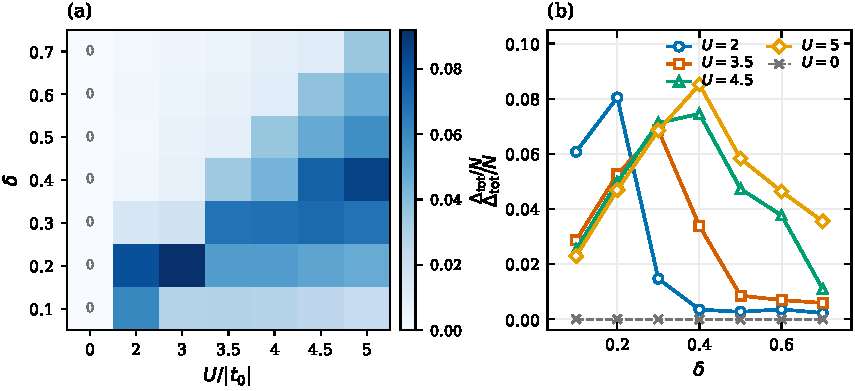
\includegraphics[width=\columnwidth]{figures/fig03_dtot_emergence}
\caption{Momentum-space spin polarization $\Delta_{\mathrm{tot}}/N$ over the $(U,\delta)$ plane at half filling, $L=12$. The $U=0$ column is identically zero at every anisotropy, which is required because the hopping in Eq.~(\ref{eq:H}) is spin independent. The signal appears only once the interaction is turned on, which is the emergent route rather than the built-in one.}
\label{fig:fig03_dtot_emergence}
\end{figure}

\begin{figure*}[tp]
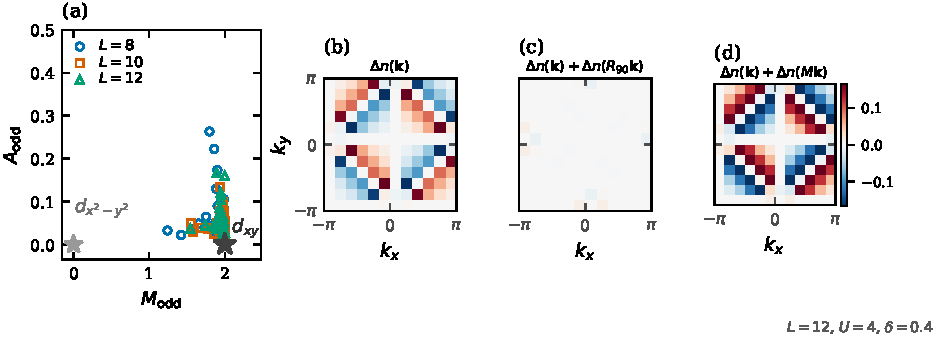
\includegraphics[width=\textwidth]{figures/fig04_symmetry}
\caption{Symmetry classification of $\Delta n(\bm{k})$ for all 126 interacting parameter sets at $L=8$, $10$ and $12$. The ratios $A_{\mathrm{odd}}$ of Eq.~(\ref{eq:aodd}) and $M_{\mathrm{odd}}$ of Eq.~(\ref{eq:modd}) place every cell at $A_{\mathrm{odd}}\simeq0$ and $M_{\mathrm{odd}}\simeq2$, which is odd under $C_4$ and even under the diagonal mirror and identifies the $d_{xy}$ channel. No cell is classified as $d_{x^2-y^2}$.}
\label{fig:fig04_symmetry}
\end{figure*}

\begin{figure*}[tp]
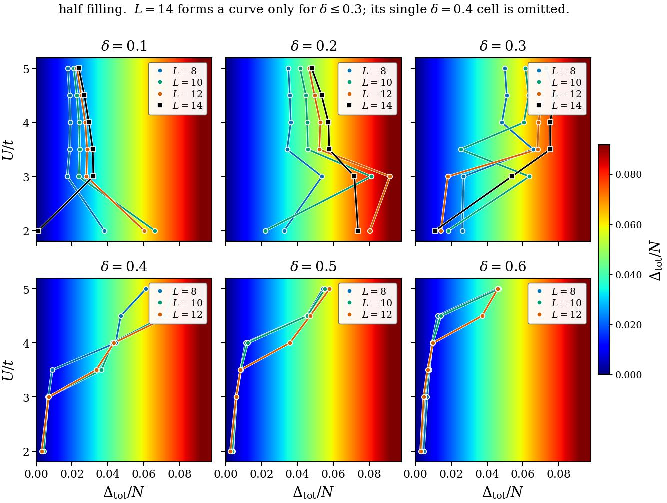
\includegraphics[width=\textwidth]{figures/fig_dtot_6delta}
\caption{$\Delta_{\mathrm{tot}}/N$ against $U$ at six anisotropies from $\delta=0.1$ to $0.6$, for $L=8$, $10$, $12$ and $14$. The background shades the value of $\Delta_{\mathrm{tot}}/N$ on the same scale as the heat maps so that the two presentations can be read against each other. $L=14$ forms a curve only for $\delta\leq0.3$.}
\label{fig:fig_dtot_6delta}
\end{figure*}

\begin{figure}[htbp]
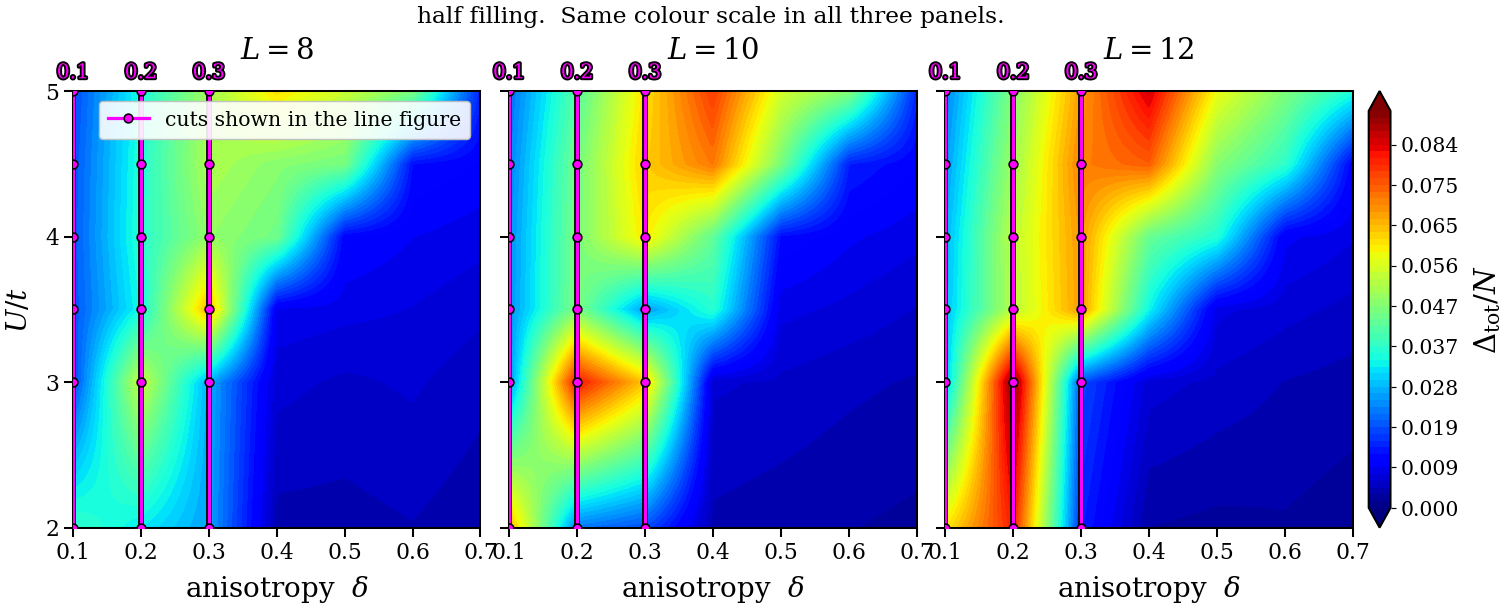
\includegraphics[width=\columnwidth]{figures/fig_dtot_maps_with_cuts}
\caption{$\Delta_{\mathrm{tot}}/N$ over the $(U,\delta)$ plane with the cuts used in the preceding figure drawn on the map, $L=12$.}
\label{fig:fig_dtot_maps_with_cuts}
\end{figure}

\begin{figure}[htbp]
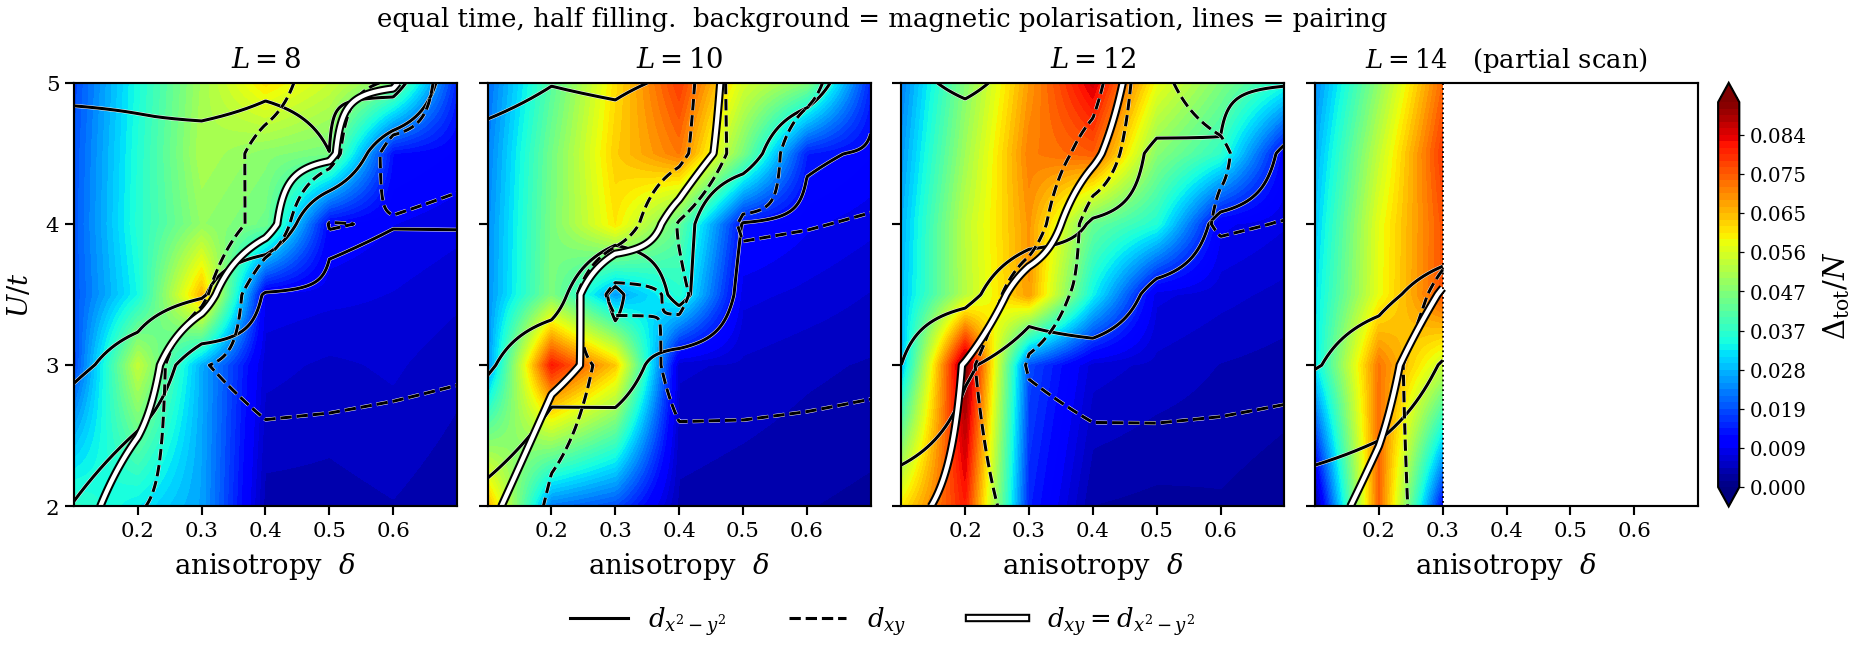
\includegraphics[width=\columnwidth]{figures/fig_overlay_4L}
\caption{The four lattice sizes overlaid, so that the size dependence of $\Delta_{\mathrm{tot}}/N$ can be read at fixed $U$ and $\delta$.}
\label{fig:fig_overlay_4L}
\end{figure}

% -------------------------------------------------------------------------
\section{Null control at vanishing anisotropy}
% ---------------------------------------------------------------------------

Equation~(\ref{eq:dtot}) sums absolute values, so statistical noise contributes
with a definite sign and $\Delta_{\mathrm{tot}}$ has a positive floor that does
not vanish when the physics requires it to. Establishing the scale of that floor
requires a calculation in which the signal is forbidden but the sampling is
unchanged.

The $U = 0$ column does not serve this purpose. There the Green function is
obtained without auxiliary fields, so the zero is a matter of arithmetic rather
than of statistics and it tests nothing about the sampling.

At $\delta = 0$ both diagonal bonds are equal on every site, the two sublattices
become equivalent, and the model reduces to the square lattice with uniform
second-neighbor hopping. Its N\'eel sublattices are related by a translation, so
$n_{\uparrow}(\bm{k}) = n_{\downarrow}(\bm{k})$ identically and
$\Delta_{\mathrm{tot}}$ must vanish by symmetry at any $U$. Whatever is measured
there is the statistical floor at production settings.

We find $\Delta_{\mathrm{tot}}/N = 6.3(2)\times10^{-4}$, averaged over
$U = 2$, $3$, $3.5$, $4$, $4.5$, and $5$ at $L = 12$.
% data/delta0_control_L12.csv: 0.000626 +/- 0.000214
At $\delta = 0.3$ the measured signal ranges from $1.47\times10^{-2}$ at
$U = 2$ to $7.13\times10^{-2}$ at $U = 4.5$, which is between $23$ and $114$
times this floor.
% data/fortran_L12_all49.csv, delta=0.3


\begin{figure}[htbp]
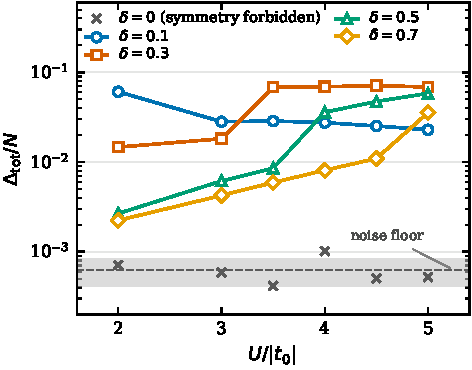
\includegraphics[width=\columnwidth]{figures/fig05_null_control}
\caption{Null control at vanishing anisotropy, logarithmic axis. At $\delta=0$ the two sublattices are related by a translation and $\Delta_{\mathrm{tot}}$ must vanish by symmetry at any $U$, so what is measured there is the statistical floor of the estimator at production settings. The floor is $6.3(2)\times10^{-4}$ per site and the measured signal at $\delta=0.3$ sits between 23 and 114 times above it.}
\label{fig:fig05_null_control}
\end{figure}

% -------------------------------------------------------------------------
\section{Finite-size behavior of the magnetic correlations}
\label{sec:fss}
% ---------------------------------------------------------------------------

The polarization of Sec.~\ref{sec:order} is measured on finite lattices, and a
nonzero value there does not by itself establish order in the thermodynamic
limit. We therefore examine two quantities that distinguish a genuine order
parameter from a finite-size remnant.

The first is the equal-time spin structure factor at the ordering wave vector,
$S(\pi,\pi)/N$. Across $L = 8$, $10$, and $12$ and for densities from
$n = 0.5$ to $n = 1$ at $U$ up to $8$, the ratio between successive sizes falls
between $0.39$ and $0.54$, against $0.44$ for a pure $1/N$ decay. A structure
factor that scales as $1/N$ carries no long-range order, so this alone leaves
the correlations short ranged on the lattices reached here.

The second is the extrapolation of the polarization to vanishing field. The
$h \to 0$ intercept of $\Delta_{\mathrm{tot}}/N$ is nonzero at each individual size and decreases
monotonically with $L$, taking the values $0.03269$, $0.02363$, $0.01845$, and
$0.01714$ at $L = 8$, $10$, $12$, and $14$. On those four points alone the
extrapolation is ambiguous. A fit in $1/L^2$ gives $\chi^2/\mathrm{dof} = 2.1$
against $7.6$ for a fit in $1/L$, which favors a finite intercept and therefore
order.

The $L = 16$ calculation resolves the ambiguity. The two fits predict $0.01325$
in $1/L$ and $0.01457$ in $1/L^2$, and the measured value is
$0.00734 \pm 0.00109$. The drop from $L = 14$ is a factor of $0.43$ where a
$1/L$ law predicts $0.88$, and including the point raises the $1/L^2$
$\chi^2/\mathrm{dof}$ from $2.1$ to $11.9$. The intercept is a finite-size
effect and the magnetic correlations remain short ranged.

This is a statement about the correlation length, not about the symmetry of the
polarization. The classification of Sec.~\ref{sec:order} rests on ratios of
sums over the Brillouin zone at a fixed lattice size, so it is unaffected by the
scaling of the correlation length.



\begin{figure*}[tp]
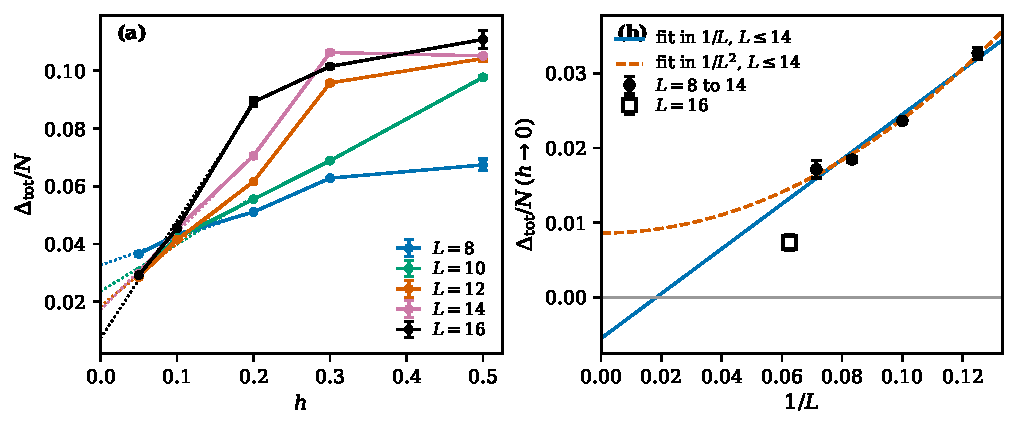
\includegraphics[width=\textwidth]{figures/fig06_fss_hscan}
\caption{(a) $\Delta_{\mathrm{tot}}/N$ against the symmetry-breaking field $h$ for $L=8$ to $16$ at $U=4$ and $\delta=0.3$, with the straight-line fits over the three smallest fields that define the $h\to0$ intercept. (b) those intercepts against $1/L$. The two curves are fits to the $L\leq14$ points alone, linear in $1/L$ and in $1/L^2$, extended to $L=16$. They predict $0.01325$ and $0.01457$ there, and the measured value is $0.00733 \pm 0.00106$. The drop from $L=14$ is a factor of $0.43$ where a $1/L$ law gives $0.88$, so the nonzero intercept seen at each individual size is a finite-size effect.}
\label{fig:fig06_fss_hscan}
\end{figure*}

\begin{figure*}[tp]
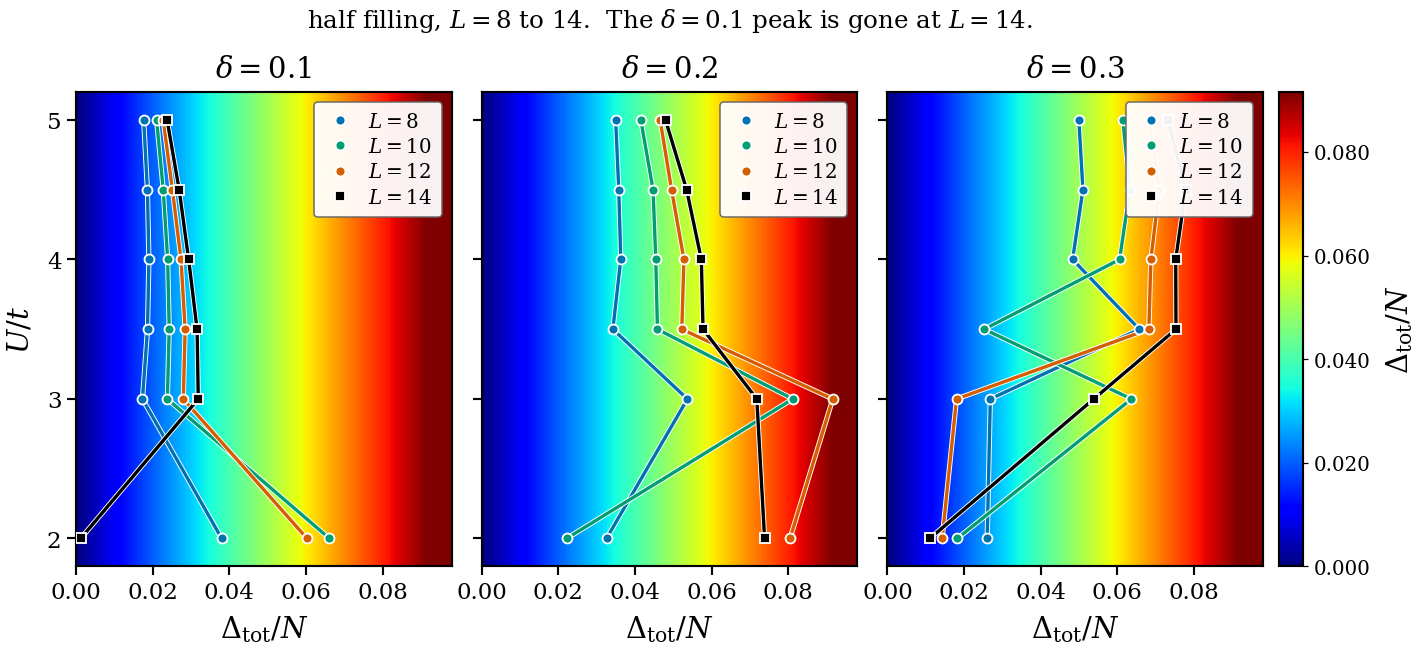
\includegraphics[width=\textwidth]{figures/fig_smallU_L8to14_bg}
\caption{Behavior at small $U$ for $\delta=0.1$, $0.2$ and $0.3$ across $L=8$ to $L=14$. The feature near $U=2$ does not survive to $L=14$ at $\delta=0.1$, where $\Delta_{\mathrm{tot}}/N$ falls to about twice the $\delta=0$ floor and the correlation with $\sin k_x \sin k_y$ is lost. At $\delta=0.3$ the decay with size is steady. The $\delta=0.2$ column persists at every size.}
\label{fig:fig_smallU_L8to14_bg}
\end{figure*}

% -------------------------------------------------------------------------
\section{Robustness and comparison}
% ---------------------------------------------------------------------------

At half filling with periodic boundaries the noninteracting gap of
Eq.~(\ref{eq:H}) is zero at every $L$ and $\delta$ we examined, so the occupied
set is fixed by the trial state rather than by the spectrum. We repeated the
calculation with antiperiodic boundaries, which shift the momentum mesh off the
high-symmetry points and open a gap, at otherwise identical settings.

The sign of $\partial \Delta_{\mathrm{tot}} / \partial U$ agrees between the two
boundary conditions at $\delta = 0.1$, where both are negative, and at
$\delta = 0.5$, where both are positive, with magnitudes matching to within a
few percent despite the different meshes. At $\delta = 0.3$ the two disagree,
and the antiperiodic value is consistent with zero. We read $\delta \approx 0.3$
as the crossover where the slope passes through zero, at which point the sign is
most sensitive to the mesh, and we therefore do not quote a slope at that
anisotropy.
% data/bc_test, analyze_bc_test.py



% -------------------------------------------------------------------------
\section{Conclusion}
The half-filled checkerboard Hubbard model supports compensated spin-split
correlations that are absent at $U=0$ and are $d_{xy}$ in symmetry at every
parameter set examined. A control at vanishing anisotropy, where the splitting is
forbidden by symmetry, places the statistical floor two orders of magnitude below
the signal, which establishes that the measured polarization is not an artifact
of the estimator or of the symmetry-broken trial state.

The mechanism uses no spin-dependent hopping and no spin-orbit coupling. It
requires only a lattice whose magnetic sublattices are related by a rotation and
a uniform Hubbard repulsion. The correlations remain short ranged on the
lattices reached here, so we do not claim long-range order, and the
constrained-path bias remains.

\appendix

% -------------------------------------------------------------------------
\section{Trial wave function and the selection of the constrained path}
\label{app:trial}
% ---------------------------------------------------------------------------

The constrained-path approximation replaces the sign problem with a bias fixed
by the trial wave function, so the trial is part of the method rather than an
implementation detail. We take the trial from an unrestricted Hartree-Fock
solution of Eq.~(\ref{eq:H}) at the same $U$, $\delta$, and filling, and we
select among the solutions reached from different starting densities by the
variational energy
\begin{equation}
E_{\mathrm{HF}} = \mathrm{Tr}\,(K \rho_{\uparrow}) + \mathrm{Tr}\,(K \rho_{\downarrow})
                + U \sum_i \langle n_{i\uparrow}\rangle \langle n_{i\downarrow}\rangle ,
\label{eq:ehf}
\end{equation}
with $\rho_{\sigma} = V_{\sigma} V_{\sigma}^{\dagger}$ built from the occupied
columns of the mean-field eigenvectors and $K$ the one-body matrix of
Eq.~(\ref{eq:H}).

Equation~(\ref{eq:ehf}) is not interchangeable with the sum of mean-field
eigenvalues. Each eigenvalue already contains the mean field of the opposite
spin, so that sum counts the interaction twice and orders competing solutions
differently from the energy. The two criteria can select different states, and
because the constrained path is fixed by whichever state is chosen, the
selection propagates into every measured quantity.

The size of the effect is not small. Selecting by the eigenvalue sum instead of
Eq.~(\ref{eq:ehf}) changes the trial in a substantial fraction of parameter
sets, and at half filling the state chosen that way carries the larger staggered
moment in every case where the two differ. We therefore report results obtained
with Eq.~(\ref{eq:ehf}) throughout.

The identity $E_{\mathrm{HF}} = \sum_p \varepsilon_p - U \sum_i \langle
n_{i\uparrow}\rangle \langle n_{i\downarrow}\rangle$ holds only at exact self
consistency and should not be substituted for Eq.~(\ref{eq:ehf}). A mean-field
iteration that mixes densities between steps does not reach that condition for
loosely converged solutions, which are precisely the ones whose ranking is at
issue.


% -------------------------------------------------------------------------
\section{Convergence in projection length}
\label{app:beta}
% ---------------------------------------------------------------------------

All results use a projection length $\beta = 32$ in units of $1/|t_0|$. Doubling
it to $\beta = 48$ at otherwise identical settings changes
$\Delta_{\mathrm{tot}}$ by between $0.1\%$ and $4.1\%$ with no systematic drift
in either direction, which we take as convergence.


% -------------------------------------------------------------------------
\section{Boundary conditions}
\label{app:bc}
% ---------------------------------------------------------------------------

At half filling with periodic boundaries the noninteracting spectrum of
Eq.~(\ref{eq:H}) is gapless at every $L$ and $\delta$ examined, so the occupied
set is fixed by the trial state rather than by the spectrum. Antiperiodic
boundaries shift the momentum mesh off the high-symmetry points and open a gap.

The sign of $\partial \Delta_{\mathrm{tot}} / \partial U$ agrees between the two
choices at $\delta = 0.1$, where both are negative, and at $\delta = 0.5$, where
both are positive, with magnitudes matching to within a few percent. At
$\delta = 0.3$ the two disagree and the antiperiodic value is consistent with
zero. We read $\delta \approx 0.3$ as the anisotropy at which the slope passes
through zero, where its sign is most sensitive to the mesh, and we do not quote
a slope there.

\begin{acknowledgments}
% TODO: funding and computing acknowledgments.
\end{acknowledgments}

\begin{thebibliography}{99}

% TODO: verify all bibliographic details before submission. Entries marked
% INCOMPLETE need the full reference supplied by the authors.

\bibitem{Smejkal2022a}
L.~\v{S}mejkal, J.~Sinova, and T.~Jungwirth,
Phys. Rev. X \textbf{12}, 031042 (2022).

\bibitem{Smejkal2022b}
L.~\v{S}mejkal, J.~Sinova, and T.~Jungwirth,
Phys. Rev. X \textbf{12}, 040501 (2022).

\bibitem{Kaushal2025}
N.~Kaushal and M.~Franz,
Phys. Rev. Lett. \textbf{135}, 156502 (2025).

\bibitem{Duerrnagel2025}
M.~D\"urrnagel \textit{et al.},
Phys. Rev. Lett. \textbf{135}, 036502 (2025);
arXiv:2412.14251.

\bibitem{OurPRB}
% INCOMPLETE: this is the group's published PRB defining Eq. (3). Full
% reference to be supplied by the authors.
[Authors], Phys. Rev. B \textbf{[vol]}, [page] ([year]).

\end{thebibliography}

\end{document}
